
% CS 111 style
% Typical usage (all UPPERCASE items are optional):
%       \input 111pre
%       \begin{document}
%       \MYTITLE{Title of document, e.g., Lab 1\\Due ...}
%       \MYHEADERS{short title}{other running head, e.g., due date}
%       \PURPOSE{Description of purpose}
%       \SUMMARY{Very short overview of assignment}
%       \DETAILS{Detailed description}
%         \SUBHEAD{if needed} ...
%         \SUBHEAD{if needed} ...
%          ...
%       \HANDIN{What to hand in and how}
%       \begin{checklist}
%       \item ...
%       \end{checklist}
% There is no need to include a "\documentstyle."
% However, there should be an "\end{document}."
%
%===========================================================
\documentclass[11pt,twoside,titlepage]{article}
%%NEED TO ADD epsf!!
\usepackage{threeparttop}
\usepackage{graphicx}
\usepackage{latexsym}
\usepackage{color}
\usepackage{listings}
\usepackage{fancyvrb}
%\usepackage{pgf,pgfarrows,pgfnodes,pgfautomata,pgfheaps,pgfshade}
\usepackage{tikz}
\usepackage[normalem]{ulem}
\tikzset{
    %Define standard arrow tip
%    >=stealth',
    %Define style for boxes
    oval/.style={
           rectangle,
           rounded corners,
           draw=black, very thick,
           text width=6.5em,
           minimum height=2em,
           text centered},
    % Define arrow style
    arr/.style={
           ->,
           thick,
           shorten <=2pt,
           shorten >=2pt,}
}
\usepackage[noend]{algorithmic}
\usepackage[noend]{algorithm}
\newcommand{\bfor}{{\bf for\ }}
\newcommand{\bthen}{{\bf then\ }}
\newcommand{\bwhile}{{\bf while\ }}
\newcommand{\btrue}{{\bf true\ }}
\newcommand{\bfalse}{{\bf false\ }}
\newcommand{\bto}{{\bf to\ }}
\newcommand{\bdo}{{\bf do\ }}
\newcommand{\bif}{{\bf if\ }}
\newcommand{\belse}{{\bf else\ }}
\newcommand{\band}{{\bf and\ }}
\newcommand{\breturn}{{\bf return\ }}
\newcommand{\mod}{{\rm mod}}
\renewcommand{\algorithmiccomment}[1]{$\rhd$ #1}
\newenvironment{checklist}{\par\noindent\hspace{-.25in}{\bf Checklist:}\renewcommand{\labelitemi}{$\Box$}%
\begin{itemize}}{\end{itemize}}
\pagestyle{threepartheadings}
\usepackage{url}
\usepackage{wrapfig}
\usepackage{hyperref}
%=========================
% One-inch margins everywhere
%=========================
\setlength{\topmargin}{0in}
\setlength{\textheight}{8.5in}
\setlength{\oddsidemargin}{0in}
\setlength{\evensidemargin}{0in}
\setlength{\textwidth}{6.5in}
%===============================
%===============================
% Macro for document title:
%===============================
\newcommand{\MYTITLE}[1]%
   {\begin{center}
     \begin{center}
     \bf
     CMPSC 300 and BIO 300 \\Introduction to Bioinformatics \\
     Fall 2017\\
     Oliver Bonham-Carter\\
     \url{http://www.cs.allegheny.edu/sites/obonhamcarter/cs300.html}
     \medskip
     \end{center}
     \bf
     #1
     \end{center}
}
%================================
% Macro for headings:
%================================
\newcommand{\MYHEADERS}[2]%
   {\lhead{#1}
    \rhead{#2}
    \immediate\write16{}
    \immediate\write16{DATE OF HANDOUT?}
    \read16 to \dateofhandout
    \lfoot{\sc Handed out on \dateofhandout}
    \immediate\write16{}
    \immediate\write16{HANDOUT NUMBER?}
    \read16 to\handoutnum
    \rfoot{Handout \handoutnum}
   }

%================================
% Macro for bold italic:
%================================
\newcommand{\bit}[1]{{\textit{\textbf{#1}}}}

%=========================
% Non-zero paragraph skips.
%=========================
\setlength{\parskip}{1ex}

%=========================
% Create various environments:
%=========================
\newcommand{\PURPOSE}{\par\noindent\hspace{-.25in}{\bf Purpose:\ }}
\newcommand{\SUMMARY}{\par\noindent\hspace{-.25in}{\bf Summary:\ }}
\newcommand{\DETAILS}{\par\noindent\hspace{-.25in}{\bf Details:\ }}
\newcommand{\HANDIN}{\par\noindent\hspace{-.25in}{\bf Hand in:\ }}
\newcommand{\SUBHEAD}[1]{\bigskip\par\noindent\hspace{-.1in}{\sc #1}\\}
%\newenvironment{CHECKLIST}{\begin{itemize}}{\end{itemize}}



\long\def\omitit #1{}

\begin{document}
\MYTITLE{Lab 1: Laboratory Assignment One: Bioinformatics Applications and BitBucket Setup.\\\color{red}Save this lab assignment to: {\tt labs/lab1}\color{black}}}
\MYHEADERS{Introduction to Bioinformatics}{Part 1 Due: 31 Aug.; Part 2 Due: 6 Sept.}{Handed out on: 30 August 2017}

\section*{Part 1: Presentations on Bioinformatics Applications}

Bioinformatics has applications in many areas of science and research.  As part of an introductory lab exercise, you and your group members will give a 5-7 minute presentation on Bioinformatics and one specific application using the questions for each application below as a guide.  Your presentation must address each of the questions and may also contain other interesting and relevant information.  Slides are not required.

\noindent  The presentations will be given during class session on 31 August, 2017. You will be given some time at the beginning of  Thursday's class session to finalize your presentation points.

\subsection*{Group 1: Diagnosing Genetic Diseases}
\begin{enumerate}
	\item What is a genetic disorder/disease (v.s. an infectious disease)?
	\item Briefly describe two genetic disorders that you have heard of.
	\item How were genetic disorders diagnosed prior to bioinformatics?
	\item How has our recent ability to sequence and analyze human genomes changed how genetic disorders can be diagnosed?  Hint: perform a Google search using the phrase ``dna testing for genetic disorder.
	\item Walk the class through an example of how bioinformatics has been used to diagnose a genetic disorder.
	\item What are some challenges facing the diagnosis of genetic disorders using bioinformatics?
	\item Based on your research, create a one sentence definition for the field of bioinformatics.
	\item Share one fun fact or interesting tidbit that your group encountered while researching genetic disorders.
\end{enumerate}

\subsection*{Group 2: Diagnosing and Tracking Infectious Disease }
\begin{enumerate}
	\item What is an infectious disease?
	\item Briefly describe two infectious diseases that you have heard of.
	\item What does it mean to track an infectious disease?
	\item How were infectious diseases diagnosed and tracked prior to bioinformatics?
	\item How has bioinformatics approaches advanced how infectious diseases can be monitored?
	\item Walk the class through an example of how bioinformatics has been used to diagnose and track an infectious disease.
	\item What are some challenges facing the infectious disease control?
	\item Based on your research, create a one sentence definition for the field of bioinformatics.
	\item Share one fun fact or interesting tidbit that your group encountered while researching infectious diseases.
\end{enumerate}

\subsection*{Group 3: Drug Discovery and Development }
\begin{enumerate}
	\item What is a drug discovery?
	\item Provide three examples of newly developed drugs that you have heard of.
	\item What are the stages in the drug discovery and development process?
	\item How were drugs discovered and developed prior to bioinformatics?
	\item How have bioinformatics approaches aided drug discovery and development?
	\item Walk the class through an example of how bioinformatics 	has been used for drug discovery and development.
	\item What are some challenges facing drug discovery and development?
	\item Based on your research, create a one sentence definition for the field of bioinformatics.
	\item Share one fun fact or interesting tidbit that your group encountered while researching drug development.
\end{enumerate}

\subsection*{Group 4: Investigating Forensic DNA evidence}
\begin{enumerate}
	\item What is forensic science?
	\item Provide two examples of different ways DNA can be used as part of a forensic investigation.
	\item How was DNA evidence analyzed prior to bioinformatics?
	\item How have bioinformatics approaches aided the analysis of DNA evidence?
	\item Walk the class through an example of how bioinformatics has aided in forensic investigations involving DNA evidence.
	\item What are some challenges facing  the analysis of DNA evidence?
	\item Based on your research, create a one sentence definition for the field of bioinformatics.
	\item Share one fun fact or interesting tidbit that your group encountered while researching forensic DNA evidence.
\end{enumerate}

\subsection*{Group 5: Understanding Metabolic Functions}
\begin{enumerate}
	\item What is metabolism?  What is a metabolic disorder?
	\item Provide three examples of metabolic disorders that you have heard of. 
	\item How were metabolic disorders studied and diagnosed prior to bioinformatics?
	\item How has bioinformatics change how metabolic disorders can be studied and diagnosed?
	\item Walk the class through an example of how bioinformatics has aided understanding metabolic functions and diagnosing disorders.
	\item What are some challenges facing the study and diagnosis of metabolic disorders?
	\item Based on your research, create a one sentence definition for the field of bioinformatics.
	\item Share one fun fact or interesting tidbit that your group encountered while researching metabolic disorders.
\end{enumerate}

\subsection*{Group 6: Improving Food Supplies}
\begin{enumerate}
	\item What is food science and technology?
	\item Provide two examples of how food science and technology has improved the world's food supply:
	\item How was food science studied prior to bioinformatics?
	\item How has bioinformatics approaches advanced the fields of food science and technology?
	\item Walk the class through an example of how bioinformatics has aided in food and nutritional research.
	\item What are some challenges facing food and nutritional research?
	\item Based on your research, create a one sentence definition for the field of bioinformatics.
	\item Share one fun fact or interesting tidbit that your group encountered while researching food science and technology.
\end{enumerate}

\subsection*{Group 7: Tailoring medical treatments to individuals (Personalized Medicine)}
\begin{enumerate}
	\item What is personalized medicine?
	\item List three disorders/diseases whose treatment has benefited from advancements in personalized medicine.
	\item How were disorders/diseases treated prior to personalized medicine (e.g., how does a doctor	determine how much and how often a drug should be administered?)?
	\item How has bioinformatics advanced the field of personalized medicine?
	\item Walk the class through an example of how bioinformatics has advanced the field of personalized medicine.
	\item What are some challenges facing personalized medicine?
	\item Based on your research, create a one sentence definition for the field of bioinformatics.
	\item Share one fun fact or interesting tidbit that your group encountered while researching personalized medicine.
\end{enumerate}

\subsection*{Group 8: Determining Evolutionary Relationships}
\begin{enumerate}
	\item What is phylogenetics?
	\item Perform a Google news search for the term ``phylogenetics''.  Briefly describe two newsworthy mentions of phylogenetics in recent years.
	\item How was phylogenetics performed prior to bioinformatics?
	\item How has bioinformatics advanced the field of phylogenetics?
	\item Walk the class through an example of how bioinformatics has advanced the field of phylogenetics.
	\item What are some challenges facing phylogenetics?
	\item Based on your research, create a one sentence definition for the field of bioinformatics.
	\item Share one fun fact or interesting tidbit that your group encountered while researching phylogenetics.
\end{enumerate}







%%%%%%


\section*{Part 2: Bitbucket Repository Set Up}

\subsection*{Objectives}
\vspace*{-.1in}
To learn how to navigate the directories within Ubuntu operating system using command line interface.~To establish and configure Bitbucket repositories that will be used in this course throughout the semester; learn basic commands for downloading course materials from the instructor and for submitting material to the instructor using Git.

\vspace*{-.2in}
\subsection*{Reading Assignment}
\vspace*{-.1in}
Please review the handout on ``Tips on Using Linux and the Command Line Interface'' and ``Bitbucket Commands''. Throughout the assignment, you should also refer to the following Web site for additional information about the Bitbucket: \url{https://confluence.atlassian.com/display/BITBUCKET/Bitbucket+101} and to find information about Git commands, please go to: \url{https://confluence.atlassian.com/stash/basic-git-commands-278071958.html} (bookmark this page).

\vspace*{-.2in}
\subsection*{Navigating using the Command Line Interface}
\vspace*{-.1in}
A command-line interface allows the user to interact with the computer by typing in commands. Computing professionals prefer to use the command line interface, built into operating systems like Linux, instead of using the graphical user interface. In many situations command line interface tends to be very efficient and effective, for example, it allows you to complete some tasks with a simple one line command instead of using the ``pumping'' motion of the mouse!
\vspace*{-.1in}
\begin{enumerate}
  \item Read through the supplemental handout on using Linux and the command line interface. As you read through the handout, follow along by trying the commands on your machine. Remember to execute a command, you should press ``Enter'' after typing a command. Check with your neighbors to see if they are able to open the terminal window, and use commands such as {\tt cd, cd .., ls}, etc.

  \item Open a terminal window on your workstation and create a directory  called {\tt cs300f2017/}  in your home directory, by typing {\tt mkdir cs300f2017/} command in your terminal.  

  \item Go to the newly created {\tt cs300f2017/} directory. Remember, the ``{\tt cd}'' command followed by the name of the directory allows you to change into a directory. Note: After you have typed in enough of the filename to specify this file from another, you can push the {\tt tab} key to automatically complete the rest of the filename.

  \item Type {\tt ls} or {\tt ls -l} command to list all of the items inside that directory. It should be empty, so nothing should appear after you type the {\tt ls} command.

  \item You can now close the terminal window by typing the {\tt exit} command. 
\end{enumerate}

\vspace*{-.2in}
\subsection*{Configuring Git and Bitbucket}
\vspace*{-.1in}
Practicing software developers normally use a version control system to manage most of the artifacts produced during the phases of the software development life cycle.  In this course, we will always use the Git distributed version control system to manage the files associated with our class, laboratory and practical sessions.  In particular, we will securely communicate with the Bitbucket.org servers that will host all of our projects.  In this laboratory assignment, we will perform all of the steps to configure the accounts on the departmental servers and the Bitbucket service.  As you will be required to use Git in the remaining laboratory and practical assignments and during the class sessions, please be sure to keep a record of all of the steps that you complete and the challenges that you face.  You are also
responsible for working with a partner to ensure that each of you is able to successfully complete each of the steps outlined in this assignment.

\begin{enumerate}

  \item If you do not already have a Bitbucket account, please go to the Bitbucket Web site and create one---make sure that you use your {\tt allegheny.edu} email address so that you can create an unlimited number of free Bitbucket repositories while you are a student. 

  \item The instructor has created the course's Bitbucket repository (repository called {\tt cs300f2017-share/}) that will be shared with you once you have created your Bitbucket account. Once the course's repository has been shared with you, Bitbucket will give you permission to clone it to have the file stored locally. To do this, open a terminal window on your workstation and change into the directory called {\tt cs300f2017/} that you created in the first portion of this assignment. %The {\tt cs300f2017/} directory will contain another repository called {\tt cs300f2017-share/} that the instructor will always use to share files with you. We install (``clone'') this new directory in the next step.
  
  \item Go to your browser where you have completed your login to Bitbucket. In the middle of the screen, under ``Overview'' you will see a command for downloading or cloning this repository/folder starting with ``git clone''.  Select HTTPS from the drop-down menu and then copy the text that is located in the text box. Back in the terminal, once you have changed into {\tt cs300f2017/} directory, please paste the bash command line code into the terminal using your mouse. If everything has worked correctly, you should be able to download all of the files that you will need for this laboratory assignment. Please resolve any problems that you encountered by first reviewing the Bitbucket documentation and then discussing the matter with the instructor.  If you are still not able to run {\tt git clone}, then please ask a peer or see the instructor.
      
  \item Using your terminal window, you should be able to browse the files that are in this shared in your {\tt Git} repository. 
  
\end{enumerate}

\vspace*{-.2in}
\subsection*{Creating a New Repository}
\vspace*{-.1in}
Now that you have learned how to clone an existing Git repository, you should make another (completely new) repository in the {\tt cs300f2017/} directory that you previously created. This new directory will be used to share your work with the instructor. 



%First, change into {\tt cs300f2017/} directory in your terminal, if you are not currently there. 



If your name were \emph{Buffalo Bill}, then your student name would be \emph{bbill}. Then inside the {\tt cs300f2017/} directory, create a new directory called {\tt cs300f2017-bbill/} using the {\tt mkdir} command in your terminal window ({\tt mkdir cs300f2017-bbill/}. If you opened a new terminal window, then you could type the following commands to create the needed directory; again, make sure that you understand each of these steps, discussing them with your neighbor, or the course instructors if you have a question.

    \vspace*{-.15in}
    \begin{verbatim}
        cd cs300f2017/
        mkdir cs300f2017-bbill/
        cd cs300f2017-bbill/
    \end{verbatim}
    \vspace*{-.33in} 

%%%%%%%%%
\omitit{
\noindent Once you have changed into this new directory you can type the command {\tt git init}.  Next, you should again use the {\tt mkdir} command to create a directory called {\tt bitbucket}. Please make sure that you completed each of these steps inside of the parent directory called {\tt cs300f2017-bbill/}.
}% end of omitit{}


\begin{figure}[!ht]
\begin{center}
%width = 8cm, height = 7.5cm
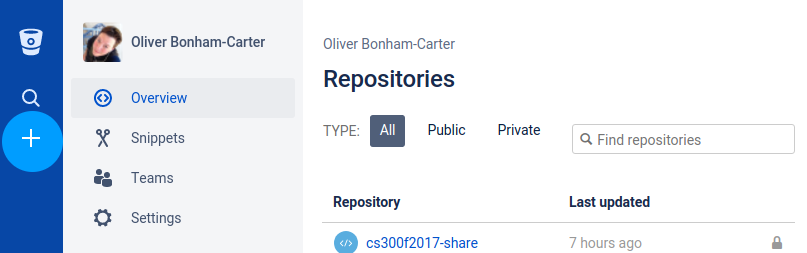
\includegraphics[scale=.5]{graphics/createButton_i.png} 
\end{center}
\caption{The button to create a repository using Bitbucket's website.}
\label{fig:createButton}
\end{figure}





\noindent In Figure \ref{fig:create} you will note the screen after you have clicked on the ``create'' command (shown in Figure \ref{fig:createButton} on Bitbucket's website. In the blank, yuo are to enter the directory name, {\tt cs300f2017-bbill/} (where you replace Buffalo Bill's ID with your own). Follow Bitbucket's instructions which will give you code for the building the repository locally and have it associated with Bitbucket's servers. Use the, \textbf{I am starting from scratch}-mode for this task. Next, give access privileges to the course instructor, (whose account is ``oliverbc'') to be able to share you work.


\noindent You can learn more about Git by consulting Web sites like \url{http://try.github.io/} and \url{http://gitimmersion.com/}. After discussing them with a class member and the instructor, you should ensure that you have a basic understanding of the following Git commands:
  % \setlength{\itemsep}{-.03in}
{\tt git init, git status, git commit, git push, git pull (used to pull over all updates from the server to your local repository} 

\begin{figure}[!ht]
\begin{center}
%width = 8cm, height = 7.5cm
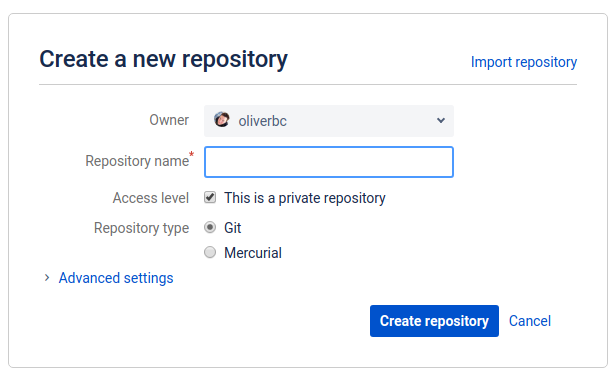
\includegraphics[scale=.5]{graphics/create.png} 
\end{center}
\caption{Fill in the name of the repository that you will create and then follow the instructions for a repository made from ``scratch''.}
\label{fig:create}
\end{figure}

\subsection*{Adding your updates to the Bitbucket server}
Once you have copied in files for your homework submission, use the following commands to push these files up to Bitbucket's cloud.

    \vspace*{-.15in}
    \begin{verbatim}
git add -A
git commit -m "Your details about the pushed files: what you added and why."
git push
    \end{verbatim}
    \vspace*{-.33in} 

Please note: Do not resubmit the data files or others, which originated in our class-shared directory. These files will likely take up massive amounts of space on the instructor's machine and departmental servers. Please locate the hidden file, {\tt .gitignore}, in the class shared directory to copy it into your own submission directory to prevent extraneous files from accidentally being pushed with the submissions of your work. Read over the {\tt .gitignore} file to determine which files are not included with each push.


%%%%%%%%%%%%%%%

\vspace*{-.2in}
\color{red}
\subsection*{Required Deliverables}
\vspace*{-.1in}
\begin{itemize}
	\item Participate in an informal presentation on the 31$^{st}$ August.
	\item Each team member is to submit a written response to the questions done by group work. Share your document with the instructor through your Bitbucket repository ({\tt cs300f2017-bbill}) by correctly using  appropriate Git commands, such as {\tt git add}, {\tt git commit -m ``your message''} and {\tt git push} to send your document to the Bitbucket's server. When you are done, please ensure that the Bitbucket Web site has
a {\tt bitbucket} directory in your repository with the required document.  
\end{itemize}
\color{black}

\noindent You should see the instructor if you have questions about assignment submission.
\end{document}
